%Chapter 2

\chapter{Objective and Literature Review}

\setlength{\belowdisplayskip}{1pt} \setlength{\belowdisplayshortskip}{1pt}
\setlength{\abovedisplayskip}{1pt} \setlength{\abovedisplayshortskip}{1pt}

\section{Objective} \label{Objective}
The objective of this report is then to apply machine learning algorithms to study an important biological process that happens during mitochondrial biogenesis. Mitochondrial biogenesis and function require the coordinated expression of both the nuclear and mitochondrial genomes \cite{Couvillion2016}. It is estimated that more than 1000 proteins make up the functional mitochondria. However, only 13 of these proteins are encoded by the mitochondrial genome and synthesized within the mitochondrial matrix.

More importantly, the oxidative phosphorylation (OXPHOS) or respiratory complexes, which are responsible for energy production are encoded by both nuclear and mitochondrial genomes. To avoid an imbalance of these subunits, the cell has to precisely coordinate the two genomes. We then want to find out how does the nuclear and mitochondrial genomes communicate with each other. There are 2 sets of data (Figure \ref{fig: Datasets}) in which each set has another subset of data (mitochondrial genes):
\begin{itemize}
	\item RNA Bulk 
	\item RNA Bulk Mito (only mitochondrial genes)
	\item RNA Crude 
	\item RNA Crude Mito (only mitochondrial genes)
\end{itemize}

\begin{figure}[H]
	\centering
	\renewcommand{\arraystretch}{0.5}
	\begin{tabular}{cc}
		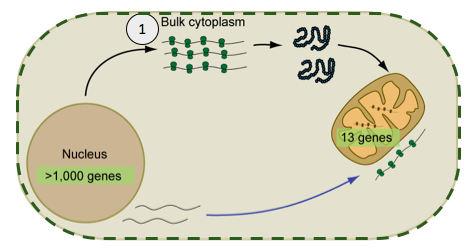
\includegraphics[width=55mm,height=35mm]{Figures/bulk.png} &
		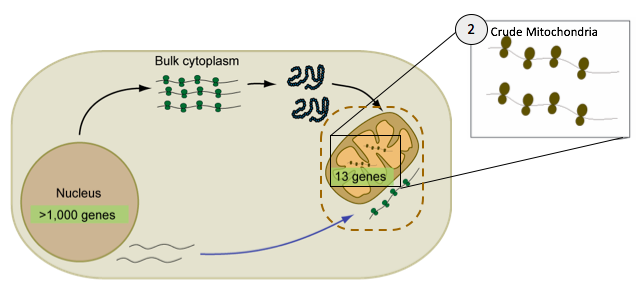
\includegraphics[width=85mm,height=55mm]{Figures/crude_mitochondria.png} \\
		Bulk Cytoplasm & Crude Mitochondria
	\end{tabular}
	\caption{Datasets}
	\label{fig: Datasets}
\end{figure}
By studying genes from these two different pools, we hope to understand the translational coordination between the nuclear and mitochondrial genomes during mitochondrial biogenesis. Specifically, the data will be in the form of expression values (numeric) of each gene at different time points.

\subsection{Clustering Gene Expression Values}
\textit{Clustering} is an exploratory data analysis technique that allows us to organize a pile of information into meaningful subgroups (\textit{clusters}) without having any prior knowledge of their group memberships. Each cluster that may arise during the analysis defines a group of objects that share a certain degree of similarity but are more dissimilar to objects in other clusters, which is why clustering is also sometimes called 'unsupervised classification'.

Clustering has many applications to computational biology. For example, we consider expression profiles of many genes taken at various developmental stages. Clustering may show that certain sets of genes line up (i.e. show the same expression levels) at various stages. This may indicate that this set of gene has common expression or regulation and we can use this to infer similar function. Furthermore, if we find a uncharacterised gene in such a set of genes, we can reason that the uncharacterised genes also has a similar function through guilt by association. 

For this project, we apply this principle which means we are working with the common assumption that genes with similar biological properties will fall under the same cluster in terms of their expression values \cite{Eisen14863}. Thus, we hope that after getting different clusters or groups of genes, each cluster may exhibit similar biological properties and distinct biological properties from one another. Afterwards, we will then be able to provide an additional information to what kind of communication or mechanism that occurs between nuclear and mitochondrial genomes.

%----------------------------------------------------------------------------------------

\section{Literature Review}
Time-series expression experiments are used to study a wide range of biological systems. More than $80\%$ of all time series expression datasets are short ($8$ time points or fewer). These dataset present unique challenges. On account of the large number of genes profiled (often tens of thousands) and the small number of time points many patterns are expected to arise at random. Most clustering algorithms are unable to distinguish between real and random patterns \cite{Ernst2005}.

Clustering algorithms have been extensively applied in the study of time-series gene expression data. Hierarchical clustering \cite{Eisen14863} and other standard clustering methods such as K-means \cite{Duda73a} are often used for this task. Furthermore, time-series data by nature or structure tends to be correlated, which can normally be dealt with the use of multivariate Gaussian mixture model \cite{Eirola}. Although these clustering algorithms have yielded many biological insights, they are not designed for time-series data, especially for short time-series. Specifically, all these methods assume that data at each time point are collected independent of each other, ignoring the sequential nature of time-series data. 

Some algorithms have been specifically modified or created to handle time-series biological data. These algorithms include clustering based on the dynamics of the expression patterns \cite{Ramoni9121}, clustering using the continuous representation of the profile \cite{Bar-Joseph} and clustering using a Hidden Markov Model (HMM) \cite{Rabiner1989, Schliep2003}. Spectral clustering \cite{Wang} has also been developed to deal with time-series data. Nonetheless, there has not been many studies done for spectral clustering and it remains an unpopular clustering algorithm for time-series data.

Furthermore, mixed-effect models or fitting cubic splines \cite{Ma2006, Golumbeanu2017, Zhang2014} to time-series expression values, which are similar to mixture model and Bayesian approach to mixture model \cite{Jia2008} have also been developed to improve the clustering of time-series data. While these algorithms work well for relatively long series dataset (10 time points or more), they are not appropriate for short time-series \cite{Ernst2005}. On account of the noise and the small number of points for each gene, most clustering algorithms cannot distinguish between patterns that occur because of random chance and clusters that represent a real response to the biological experiment. Short Time-series Expression Miner (STEM) \cite{Ernst2005} is one commonly used algorithm to deal with this problem due to the way it is constructed and its success in producing biologically significant clusters.

Nevertheless, the study of clustering algorithm for time-series data is still inconclusive which means that it may still ultimately depend on the nature of the data itself. For instance, hierarchical clustering remains a popular choice for clustering gene time-series expression values despite its failure for some cases. Hence, other than applying STEM in our report, we will still study popular clustering algorithms such as Gaussian Mixture Model, K-means and Hierarchical Clustering.